
\subsection{Métodos empíricos para análise de vazamentos}

%% \erick[inline]{usar paper e slides SPACE e slides talk at Riscure ~\cite{GoodwillJun2011, WittemanJaffe2013, TunstallGoodwill2016}}

Avaliações de segurança de dispositivos criptográficos com respeito a canais laterais compreende duas fases: \textit{medição} e \textit{análise}.
%
A saída ou resultado de tal avaliação deve Falhou (\textit{Fail}) ou Passou (\textit{Pass}). 
%
O resultado de tal avaliação deve ser interpretado segundo as restrições do processo de avaliação, tais como a acurácia do equipamento de teste, expertise técnica dos avaliadores e tempo disponível para a avaliação.
%
A medição dos traces e suas limitações deve ser levada em consideração, caso contrário a fase posterior, de análise, pode ser prejudicada ou invalidada, resultando em falsos positivos, ou pior, em falsos negativos.
%%
%%

As metodologias de avaliação atuais (p.ex., Common Criteria~\cite{CommonCriteria2014}) consistem na realização de um bateria de ataques por canais laterais conhecidos contra o dispositivo sob teste (DUT)~\footnote{Device under test.} em uma tentativa de recuperar a chave. Apesar disto, a rápida evolução das técnicas de análise por canais laterais atuais propostas na literatura incorrem em ambos um nível crescente de expertise dos testadores e um crescimento no tempo requerido para avaliação. Mesmo quando todas as tentativas de ataque falham, vazamentos residuais no canal lateral avaliado podem ainda estar presentes, o que pode revelar novos caminhos de ataque (\textit{attack paths}) para um adversário.
%
%For these reasons, NIST organized a workshop~\cite{NIST_NIAT_2011} to encourage the development of test methods, metrics and tools for evaluating the effectiveness of mitigations against non-invasive attacks on cryptographic modules.
%%
%%

\subsubsection{Test Vector Leakage Assessment (TVLA)}\label{sec-tvla}

Por estas razões o NIST organizou um workshop em 2011~\cite{NIST_NIAT_2011} para encorajar o desenvolvimento de métodos de teste, métricas e ferramentas para avaliação da eficácia de mitigações contra ataques não-invasivos à módulos criptográficos.

% cRI proposed the Test Vector Leakage Assessment (TVLA) testing methodology, to solve the aforementioned issues, which is claimed to be effective, in the sense that it is reproducible and is a reliable indicator of the resistance achieved, and cost effective, meaning that ``validating a moderate level of resistance (e.g., FIPS 140 level 3 or 4) should not require an excessive amount of testing time per algorithm or test operator skills"~\cite{Goodwill2011}. Their approach differs fundamentally from the attack-focused evaluation strategies currently employed, taking a black-box and detection-focused strategy~\cite{MatherOswaldBandenburg2013}.

Neste workshop a CRI\footnote{Empresa ``Cryptography Research'', atualmente incorporada à Rambus.} propôs a metodologia \textit{Test Vector Leakage Assessment} (TVLA)~\cite{Goodwill2011} com o propósito de resolver os problemas acima. Os autores desta metodologia consideram duas figuras de mérito são importantes, a eficácia, no sentido de que ela é reprodutível e é um indicador confiável da resistência atingida pelo dispositivo, e a relação custo-benefício, isto é, na palavra dos autores, ``validar um nível moderado de resistência (p.ex., FIPS 140 nível 3 ou 4) não deve requerer uma quantidade excessiva de tempo de teste por algoritmo ou de habilidade do operador de teste''~\cite{Goodwill2011}. A abordagem da metodologia TVLA difere fundamentalmente das estratégias de avaliação focadas em ataque atualmente empregadas, adotando uma estratégia caixa-preta com foco na detecção de vazamento.

% cRI's methodology measurement phase is based on the collection of side-channel traces when standardized test vectors are provided as input to the algorithm implementation being tested, and establishes requirements for power measurement equipment and setup, data collection, signal alignment and preprocessing. 
A fase de medição na TVLA é baseada na aquisição de traces de canal lateral quando vetores de teste padronizados são fornecidos como entrada para a implementação sob teste, e estabelece requisitos para os equipamentos e setup de medição, alinhamento e preprocessamento dos traces.

% The analysis phase comprises statistical hypothesis testing, more specifically, Welch's $t$-test, which is able to detect different types of leakages and allows the analyst to identify points in time that deserve further investigation. 
A fase de análise compreende teste de hipótese estatístico, mais especificamente, o $t$-test de Welch, o qual é capaz de detectar diferentes tipos de vazamento e permite ao analista identificar pontos no tempo que merecem investigação adicional.

% The testing methodology has so far been applied to AES hardware and software implementations (by the proposal authors~\cite{Goodwill2011,Cooper2013} and independently~\cite{MatherOswaldBandenburg2013}), and RSA software implementations~\cite{Witteman2011}.
A metodologia TVLA até então foi aplicada à implementações do AES em hardware e software~\cite{Goodwill2011,Cooper2013,MatherOswaldBandenburg2013}, e implementações em software do RSA~\cite{Witteman2011} e ECC (multiplicação escalar com base variável)~\cite{Nascimento2015_Space}. Bem recentemente, os autores da TVLA detalharam mais a aplicação da metodologia ao RSA e como adaptá-la aos esquemas ECDSA e ECDH.~\cite{TunstallGoodwill2016}.

\subsubsection{Outras metodologias para análise de vazamentos}

%Other methodologies, based on continuous~\cite{Chothia2011} and discrete~\cite{Chatzikokolakis2010} mutual information have also been proposed.
%
Outras metodologias, baseadas em informação mútua contínua~\cite{Chothia2011} e discreta~\cite{Chatzikokolakis2010} também foram propostas.
%
%Oswald et al~\cite{MatherOswaldBandenburg2013} analyzed methodologies~\cite{Goodwill2011},~\cite{Chatzikokolakis2010} and ~\cite{Chothia2011}, and concluded they have similar statistical power.
%
Oswald et al~\cite{MatherOswaldBandenburg2013} analisaram as metodologias~\cite{Goodwill2011},~\cite{Chatzikokolakis2010} e ~\cite{Chothia2011}, e concluiu que elas tem poder estatístico similar.
%
%The recent work of Schneider and Moradi~\cite{SchneiderMoradi2015} address how to perform the $t$-test in~\cite{Goodwill2011} at higher orders, and how to extend it to multivariate settings.
%
O trabalho recente de Schneider e Moradi~\cite{SchneiderM16} aborda como realizar o teste $t$ em~\cite{Goodwill2011} em ordens mais altas e como estendê-lo para o contexto multivariado.
%
\subsubsection{Aplicação da metodologia TVLA para ECC}

% We show the application of CRI's methodology to an implementation of ECDH-Curve25519 for the AVR microcontroller~\cite{Nascimento2015_Space}. 
%
Nesta subseção nós mostramos a aplicação da metodologia TVLA à um implementação para microcontrolador AVR do esquema ECDH utilizando a curva Curve25519 e o algoritmo Montgomery Ladder para ECSM protegida com a contramedida de aleatorização de coordenadas projetivas (CR)~\cite{Nascimento2015_Space}.
%
% Specifically, we select a set of test vectors (Table \ref{tbSetsTVs}) to be used for the power measurement phase, which cover normal and special cases of the field and group arithmetic when implemented using the chosen algorithms. 
Especificamente, os conjuntos de vetores de teste na ~\Cref{tbSetsTVs}) foram selecionados para serem usados para a fase de medição de consumo de potência, os quais cobrem casos normais e especiais da aritmética de corpo finito e de grupo.
%
% Table \ref{tbSpecialValuesECDH} shows categories of special values used in Sets $4$ and $5$ for the compute shared secret function.
%
A~\Cref{tbSpecialValuesECDH} mostra categorias de valores especiais usados nos conjuntos 4 e 5 para a função compute shared secret do esquema ECDH-Curve25519.

\begin{table}[htb]\scriptsize
	\caption{Conjuntos de vetores de teste para análise de vazamento SPA ($k$ é um escalar secreto e $P$ é um ponto).}
	\label{tbSetsTVs}
	%\resizebox{1.0\textwidth}{!} { \begin{minipage}{\textwidth}
	\centering%\begin{center}
	\bgroup
	\def\arraystretch{\tblvertpaddingfactor} %cell vertical padding
	\setlength{\tabcolsep}{\tblhorizpadding} %cell horizontal padding
	\begin{tabular}{|c|c|c|} 	%\begin{tabular}{|c|c|m{0.5\textwidth}|}
		\hline 
		\# Conj.	& Propriedades	& Descrição \\ \hline \hline
		1		& $k$ constante, $P$ constante	&	Este é o baseline. Os testes comparam os traces dos outros conjuntos contra este. \\ \hline 
		2		& $k$ constante, $P$ varia	&	Meta é detectar relações sistemáticas entre consumo de potência e o valor de $P$. %Goal is to detect systematic relationships between power consumption and the $P$ value. 
		\\ \hline 
		3		& $k$ varia, $P$ constante	&	Meta é detectar relações sistemáticas entre consumo de potência e o valor de $k$. \\ \hline  %Goal is to detect systematic relationships between power consumption and the $k$ value.
		4		& $k$ constante, $P$ especial	&	Casos de borda dos algoritmos utilizados. \\ \hline %Edge cases of the algorithms used.		 
		5		& $k$ especial, $P$ constante	&	Casos de borda dos algoritmos utilizados. %Edge cases of the algorithms used.
		\\ \hline
	\end{tabular}
	\egroup
	%\end{center}%\end{minipage} }
\end{table}

\begin{table}[htb]\scriptsize
	\caption{Categorias de valores especiais para $n$ e $q$ na função compute shared secret em ECDH-Curve25519 ($q$ é um ponto codificado, $n$ é um escalar codificado e $l$ é a ordem do subgrupo).}
	\label{tbSpecialValuesECDH}
	%\resizebox{1.0\textwidth}{!} { \begin{minipage}{\textwidth}
	\begin{center}
		\bgroup
		\def\arraystretch{\tblvertpaddingfactor} %cell vertical padding
		\setlength{\tabcolsep}{\tblhorizpadding} %cell horizontal padding
		\begin{tabular}{|c|l|}
			\hline
			Cat. \#	& Propriedades	\\ \hline \hline
			1		& $q \in \{0,1,...,1023\}$	\\ \hline 
			2		& $q \in \{p_{25519}-1,...,p_{25519}-1024\}$	\\ \hline 
			3		& $n \in \{0,...,1023\}$	\\ \hline
			4		& $n \in \{l-1,...,l-1024\}$	\\ \hline 
			5		& $q$ tem um alto peso de Hamming ($\geq 230$) \\ \hline
			6		& $q$ tem um baixo peso de Hamming ($\leq 25$) \\ \hline
		\end{tabular}
		\egroup
	\end{center} 
	%\end{minipage} }
\end{table}

% We obtained 200 average traces for each test vector set, for a total of 1000 traces. 
%
\noindent \textbf{Fase de aquisição}. Os autores~\cite{Nascimento2015_Space} capturaram 200 traces de potência para cada um dos conjuntos de vetores de teste, totalizando 1000 traces.
%
\begin{comment}
The leakage analysis phase of our implementation of ECDH-Curve25519 with randomized coordinates countermeasure is identical to CRI's TVLA~\cite{Witteman2011}, and is conducted in the following way. Let $\{DS_1,\ldots,DS_5\}$ be the sets of power traces corresponding to the selected test vectors sets.
\end{comment}
%
A fase de análise de vazamento é idêntica à proposta na metodologia TVLA para o RSA~\cite{Witteman2011}, e é conduzida da seguinte forma. Sejam $\{DS_1,\ldots,DS_5\}$ os conjuntos de traces de potência correspondentes aos conjuntos de vetores de teste selecionados.
%
\begin{comment}
The full test consists of running the (pairwise) tests described in~\cite{Witteman2011} for each of the following pairs of datasets: $\{(DS_1,DS_2)$, \dots, $(DS_1,DS_5) \}$.
\end{comment}
%

O teste completo consiste em executar os testes pareados descritos em~\cite{Witteman2011} para cada um dos seguintes pares de datasets: $\{(DS_1,DS_2)$, \dots, $(DS_1,DS_5) \}$.
%
\begin{comment}
If any of the previous tests fails, then the top-level test fails and the implementation is deemed to have FAILED. Otherwise, it PASSED. We chose the confidence threshold $C = 4.5$, the same value used in CRI's methodology for RSA~\cite{Witteman2011}.
\end{comment}
%
Se qualquer um dos testes anteriores falha, então o resultado da avaliação da implementação é~\textit{FALHOU}. Caso contrário, o resultado é~\textit{PASSOU}. Nós escolhemos o limiar de confiança $C = 4.5$, o mesmo valor usado na metodologia TVLA para o RSA~\cite{Witteman2011}.
%
% \textbf{SPA Analysis.} The leakage analysis methodology was applied to our implementation of ECDH-Curve25519 with randomized coordinates. ~\Cref{fig:graph__t_statistic__x__sample_index_for_groups_A_and_B__pair_DS1_DS3} shows the $t$-statistic for a small range of sample indices
%

\noindent \textbf{Fase de análise SPA}. A ~\Cref{fig:graph__t_statistic__x__sample_index_for_groups_A_and_B__pair_DS1_DS3} mostra a estatística $t$ para um pequeno intervalo de índices de amostra.
%
%\footnote{This time interval was selected because it illustrates a range where the $t$-statistic values are relatively high, compared to other time instants.} (time instants), 
%
\footnote{Este intervalo de tempo foi selecionado porque ele ilustra um intervalo onde os valores da estatística $t$ são altos comparados com os os instantes de tempo} (i.e., time instants),
%
% for one run of Welch's $t$-test for group A $(S_{A,1},S_{A,2})$ of vectors selected from $DS_1$ and $DS_3$, and the same test run over the independent group B $(S_{B,1},S_{B,2})$.
%
para uma execução do teste $t$ para grupo A $(S_{A,1},S_{A,2})$ de vetores selecionados de $DS_1$ e $DS_3$, e o mesmo teste executado sobre o grupo (independente) B $(S_{B,1},S_{B,2})$.
%
%\footnote{Groups A and B are a partition of test vector sets $DS_1$ and $DS_3$: $(S_{A,1}\subset DS_1,\ \  S_{A,2}\subset DS_3)$ and $(S_{B,1} = DS_1\setminus S_{A,1},\ \ S_{B,2} = DS_3\setminus S_{A,2})$.} 
%
\footnote{Os grupos A e B são uma partição dos conjuntos de vetores de teste $DS_1$ e $DS_3$: $(S_{A,1}\subset DS_1,\ \  S_{A,2}\subset DS_3)$ e $(S_{B,1} = DS_1\setminus S_{A,1},\ \ S_{B,2} = DS_3\setminus S_{A,2})$.} 
%
% The $t$-statistic for group A is above $C = 4.5$ at one time instant, meaning a possible strong dependence between power consumption and key value at that instant. But, as it did not occur at the same time and in the same direction for group B, it is therefore considered a false positive by the methodology and thus discarded. 
%

A estatística $t$ para grupo A está acima do limiar $C = 4.5$ em um instante de tempo, significando uma possível dependência forte entre o consumo de potência e o valor da chave naquele instante. Mas, como este evento não ocorreu ao mesmo tempo e na mesma direção para o grupo B, ele é considerado um falso positivo pelo metodologia e assim é descartado.
%
%The test results for each pair of test vector sets $ \{(DS_1,DS_2), \dots, (DS_1,DS_5) \}$ showed that at a few time instants the $t$-statistic value for one of the groups is above $4.5$ or below $-4.5$, but not for both groups at the same time. 
%

Os resultados de teste para cada par de conjuntos de vetores de teste $ \{(DS_1,DS_2), \dots, (DS_1,DS_5) \}$ mostrou que em poucos instantes de tempo o valor da estatística $t$ para um dos grupos esteve acima de $4.5$ ou abaixo de $-4.5$, mas nunca para ambos os grupos ao mesmo tempo.
%Therefore, we can conclude that our SPA protected implementation of ECDH-Curve25519 passed the SPA leakage evaluation.
%
Portanto, pode-se concluir que a implementação passou a avaliação de vazamento SPA segundo a metodologia TVLA.

\begin{figure}[htb]
	\centering
	\centerline{
		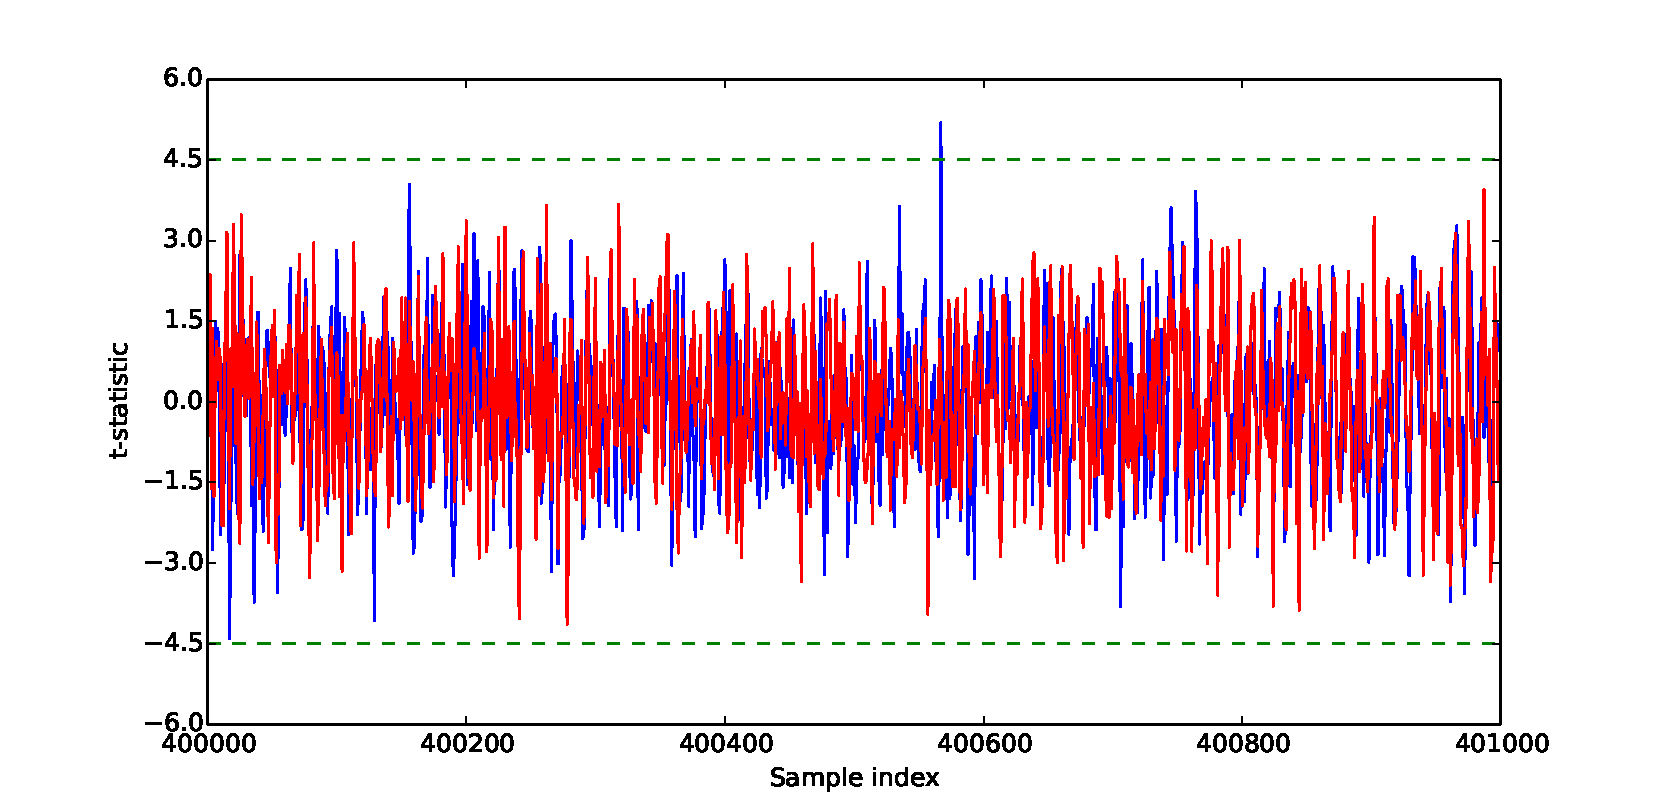
\includegraphics[width=1.1\textwidth]{figures/graph__t_statistic__x__sample_index_for_groups_A_and_B__pair_DS1_DS3-eps-converted-to.pdf}
	}
	\caption{$t$-statistic versus sample index for the experiment comparing $DS_1$ and $DS_3$, for two independent groups of traces; group A (blue) and group B (red).}
	\label{fig:graph__t_statistic__x__sample_index_for_groups_A_and_B__pair_DS1_DS3}
\end{figure}